\documentclass{standalone}
\usepackage{tikz}
\usetikzlibrary{patterns, positioning}


\begin{document}
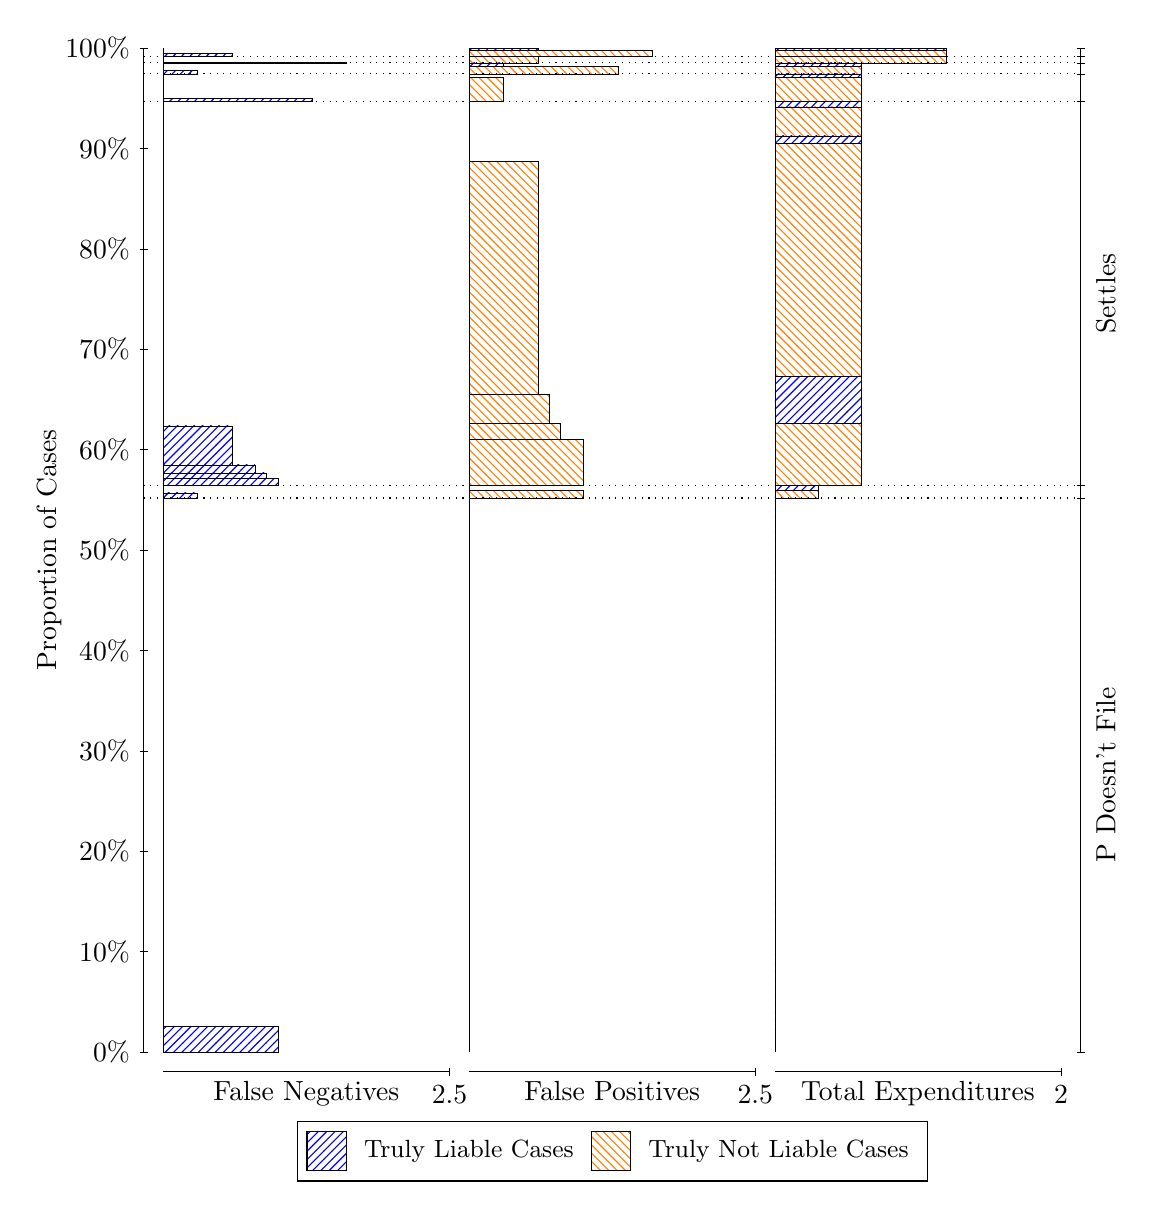
\begin{tikzpicture}
\draw[black, very thin] (1.5,1.75) -- (1.5,14.5);
\node[rotate=90, text=black, anchor=center] at (0.3, 8.125) {Proportion of Cases};
\draw[black, very thin] (1.45,1.75) -- (1.55,1.75);
\node[text=black, anchor=east] at (1.45, 1.75) {0\%};
\draw[black, very thin] (1.45,3.025) -- (1.55,3.025);
\node[text=black, anchor=east] at (1.45, 3.025) {10\%};
\draw[black, very thin] (1.45,4.3) -- (1.55,4.3);
\node[text=black, anchor=east] at (1.45, 4.3) {20\%};
\draw[black, very thin] (1.45,5.575) -- (1.55,5.575);
\node[text=black, anchor=east] at (1.45, 5.575) {30\%};
\draw[black, very thin] (1.45,6.85) -- (1.55,6.85);
\node[text=black, anchor=east] at (1.45, 6.85) {40\%};
\draw[black, very thin] (1.45,8.125) -- (1.55,8.125);
\node[text=black, anchor=east] at (1.45, 8.125) {50\%};
\draw[black, very thin] (1.45,9.4) -- (1.55,9.4);
\node[text=black, anchor=east] at (1.45, 9.4) {60\%};
\draw[black, very thin] (1.45,10.675) -- (1.55,10.675);
\node[text=black, anchor=east] at (1.45, 10.675) {70\%};
\draw[black, very thin] (1.45,11.95) -- (1.55,11.95);
\node[text=black, anchor=east] at (1.45, 11.95) {80\%};
\draw[black, very thin] (1.45,13.225) -- (1.55,13.225);
\node[text=black, anchor=east] at (1.45, 13.225) {90\%};
\draw[black, very thin] (1.45,14.5) -- (1.55,14.5);
\node[text=black, anchor=east] at (1.45, 14.5) {100\%};

\draw[black, very thin] (13.4,1.75) -- (13.4,14.5);
\draw[black, very thin] (13.35,1.75) -- (13.45,1.75);
\node[anchor=west] at (13.35, 1.75) {};
\draw[black, very thin] (13.35,8.7861) -- (13.45,8.7861);
\node[anchor=west] at (13.35, 8.7861) {};
\draw[black, very thin] (13.35,8.9437) -- (13.45,8.9437);
\node[anchor=west] at (13.35, 8.9437) {};
\draw[black, very thin] (13.35,13.819) -- (13.45,13.819);
\node[anchor=west] at (13.35, 13.819) {};
\draw[black, very thin] (13.35,14.172) -- (13.45,14.172);
\node[anchor=west] at (13.35, 14.172) {};
\draw[black, very thin] (13.35,14.312) -- (13.45,14.312);
\node[anchor=west] at (13.35, 14.312) {};
\draw[black, very thin] (13.35,14.397) -- (13.45,14.397);
\node[anchor=west] at (13.35, 14.397) {};
\draw[black, very thin] (13.35,14.5) -- (13.45,14.5);
\node[anchor=west] at (13.35, 14.5) {};

\draw[black, very thin, pattern color=blue, pattern=north east lines] (1.75,1.75) rectangle (3.2033,2.0787);
\draw[black, very thin, pattern color=orange, pattern=north west lines] (1.75,2.0787) rectangle (1.75,8.7861);
\draw[black, very thin, pattern color=blue, pattern=north east lines] (1.75,8.7861) rectangle (2.186,8.8496);
\draw[black, very thin, pattern color=orange, pattern=north west lines] (1.75,8.8496) rectangle (1.75,8.9437);
\draw[black, very thin, pattern color=blue, pattern=north east lines] (1.75,8.9437) rectangle (3.2033,9.0389);
\draw[black, very thin, pattern color=blue, pattern=north east lines] (1.75,9.0389) rectangle (3.058,9.1043);
\draw[black, very thin, pattern color=blue, pattern=north east lines] (1.75,9.1043) rectangle (2.9127,9.2067);
\draw[black, very thin, pattern color=blue, pattern=north east lines] (1.75,9.2067) rectangle (2.622,9.7009);
\draw[black, very thin, pattern color=orange, pattern=north west lines] (1.75,9.7009) rectangle (1.75,13.819);
\draw[black, very thin, pattern color=blue, pattern=north east lines] (1.75,13.819) rectangle (3.6393,13.863);
\draw[black, very thin, pattern color=orange, pattern=north west lines] (1.75,13.863) rectangle (1.75,14.172);
\draw[black, very thin, pattern color=blue, pattern=north east lines] (1.75,14.172) rectangle (2.186,14.215);
\draw[black, very thin, pattern color=orange, pattern=north west lines] (1.75,14.215) rectangle (1.75,14.312);
\draw[black, very thin, pattern color=blue, pattern=north east lines] (1.75,14.312) rectangle (4.0753,14.32);
\draw[black, very thin, pattern color=orange, pattern=north west lines] (1.75,14.32) rectangle (1.75,14.397);
\draw[black, very thin, pattern color=blue, pattern=north east lines] (1.75,14.397) rectangle (2.622,14.428);
\draw[black, very thin, pattern color=orange, pattern=north west lines] (1.75,14.428) rectangle (1.75,14.5);
\draw[black, very thin, pattern color=orange, pattern=north west lines] (5.6333,1.75) rectangle (5.6333,8.4574);
\draw[black, very thin, pattern color=blue, pattern=north east lines] (5.6333,8.4574) rectangle (5.6333,8.7861);
\draw[black, very thin, pattern color=orange, pattern=north west lines] (5.6333,8.7861) rectangle (7.0867,8.8802);
\draw[black, very thin, pattern color=blue, pattern=north east lines] (5.6333,8.8802) rectangle (5.6333,8.9437);
\draw[black, very thin, pattern color=orange, pattern=north west lines] (5.6333,8.9437) rectangle (7.0867,9.5343);
\draw[black, very thin, pattern color=orange, pattern=north west lines] (5.6333,9.5343) rectangle (6.796,9.7314);
\draw[black, very thin, pattern color=orange, pattern=north west lines] (5.6333,9.7314) rectangle (6.6507,10.1);
\draw[black, very thin, pattern color=orange, pattern=north west lines] (5.6333,10.1) rectangle (6.5053,13.062);
\draw[black, very thin, pattern color=blue, pattern=north east lines] (5.6333,13.062) rectangle (5.6333,13.819);
\draw[black, very thin, pattern color=orange, pattern=north west lines] (5.6333,13.819) rectangle (6.0693,14.128);
\draw[black, very thin, pattern color=blue, pattern=north east lines] (5.6333,14.128) rectangle (5.6333,14.172);
\draw[black, very thin, pattern color=orange, pattern=north west lines] (5.6333,14.172) rectangle (7.5227,14.27);
\draw[black, very thin, pattern color=blue, pattern=north east lines] (5.6333,14.27) rectangle (6.0693,14.312);
\draw[black, very thin, pattern color=orange, pattern=north west lines] (5.6333,14.312) rectangle (6.5053,14.389);
\draw[black, very thin, pattern color=blue, pattern=north east lines] (5.6333,14.389) rectangle (5.6333,14.397);
\draw[black, very thin, pattern color=orange, pattern=north west lines] (5.6333,14.397) rectangle (7.9587,14.469);
\draw[black, very thin, pattern color=blue, pattern=north east lines] (5.6333,14.469) rectangle (6.5053,14.5);
\draw[black, very thin, pattern color=orange, pattern=north west lines] (9.5167,1.75) rectangle (9.5167,8.4574);
\draw[black, very thin, pattern color=blue, pattern=north east lines] (9.5167,8.4574) rectangle (9.5167,8.7861);
\draw[black, very thin, pattern color=orange, pattern=north west lines] (9.5167,8.7861) rectangle (10.062,8.8802);
\draw[black, very thin, pattern color=blue, pattern=north east lines] (9.5167,8.8802) rectangle (10.062,8.9437);
\draw[black, very thin, pattern color=orange, pattern=north west lines] (9.5167,8.9437) rectangle (10.607,9.7314);
\draw[black, very thin, pattern color=blue, pattern=north east lines] (9.5167,9.7314) rectangle (10.607,10.328);
\draw[black, very thin, pattern color=orange, pattern=north west lines] (9.5167,10.328) rectangle (10.607,13.289);
\draw[black, very thin, pattern color=blue, pattern=north east lines] (9.5167,13.289) rectangle (10.607,13.384);
\draw[black, very thin, pattern color=orange, pattern=north west lines] (9.5167,13.384) rectangle (10.607,13.753);
\draw[black, very thin, pattern color=blue, pattern=north east lines] (9.5167,13.753) rectangle (10.607,13.819);
\draw[black, very thin, pattern color=orange, pattern=north west lines] (9.5167,13.819) rectangle (10.607,14.128);
\draw[black, very thin, pattern color=blue, pattern=north east lines] (9.5167,14.128) rectangle (10.607,14.172);
\draw[black, very thin, pattern color=orange, pattern=north west lines] (9.5167,14.172) rectangle (10.607,14.27);
\draw[black, very thin, pattern color=blue, pattern=north east lines] (9.5167,14.27) rectangle (10.607,14.312);
\draw[black, very thin, pattern color=orange, pattern=north west lines] (9.5167,14.312) rectangle (11.697,14.389);
\draw[black, very thin, pattern color=blue, pattern=north east lines] (9.5167,14.389) rectangle (11.697,14.397);
\draw[black, very thin, pattern color=orange, pattern=north west lines] (9.5167,14.397) rectangle (11.697,14.469);
\draw[black, very thin, pattern color=blue, pattern=north east lines] (9.5167,14.469) rectangle (11.697,14.5);
\draw[black, dotted] (1.5,8.7861) -- (13.4,8.7861);
\draw[black, dotted] (1.5,8.9437) -- (13.4,8.9437);
\draw[black, dotted] (1.5,13.819) -- (13.4,13.819);
\draw[black, dotted] (1.5,14.172) -- (13.4,14.172);
\draw[black, dotted] (1.5,14.312) -- (13.4,14.312);
\draw[black, dotted] (1.5,14.397) -- (13.4,14.397);
\draw[black, very thin] (1.75,1.5) -- (5.3833,1.5);
\node[text=black, anchor=north] at (3.5667, 1.5) {False Negatives};
\draw[black, very thin] (5.3833,1.45) -- (5.3833,1.55);
\node[text=black, anchor=north] at (5.3833, 1.45) {2.5};

\draw[black, very thin] (5.6333,1.5) -- (9.2667,1.5);
\node[text=black, anchor=north] at (7.45, 1.5) {False Positives};
\draw[black, very thin] (9.2667,1.45) -- (9.2667,1.55);
\node[text=black, anchor=north] at (9.2667, 1.45) {2.5};

\draw[black, very thin] (9.5167,1.5) -- (13.15,1.5);
\node[text=black, anchor=north] at (11.333, 1.5) {Total Expenditures};
\draw[black, very thin] (13.15,1.45) -- (13.15,1.55);
\node[text=black, anchor=north] at (13.15, 1.45) {2};

\node[text=black, centered, rotate=90] at (13.72, 5.268) {P Doesn't File};

\node[text=black, centered, rotate=90] at (13.72, 11.381) {Settles};





\draw (7.449999999999999,1.5) node[draw=none] (baseCoordinate) {};
\begin{scope}[align=center]
        \matrix[scale=0.5, draw=black, below=0.5cm of baseCoordinate, nodes={draw}, column sep=0.1cm]{
            \node[rectangle, draw, minimum width=0.5cm, minimum height=0.5cm, pattern color=blue, pattern=north east lines] {}; &
            \node[draw=none, font=\small, text=black] (B) {Truly Liable Cases}; &
            \node[rectangle, draw, minimum width=0.5cm, minimum height=0.5cm, pattern color=orange, pattern=north west lines] {}; &
            \node[draw=none, font=\small, text=black] (B) {Truly Not Liable Cases}; \\
            };
\end{scope}

\end{tikzpicture}
\end{document}